\documentclass{beamer}
\usepackage[utf8]{inputenc}
\usepackage[T1]{fontenc}
\usepackage{lmodern}
\usepackage{graphicx}
\usepackage{amsmath,amsfonts,amssymb}
\usepackage{tikz}

\begin{document}
  \title{Opam for Coq}
  \author{Guillaume Claret}
  \date{October 23, 2014 - Coq Working Group}
  \maketitle

  \begin{frame}
    \frametitle{The need for a package manager}
    \begin{itemize}
      \item few user developments are reused
      \item \emph{contribs} mechanism, but outdated and centralized
      \item no simple / uniform way to install a foreign library
      \item even if there seem to be more and more developers...
    \end{itemize}
    A lot of time is lost. What other programming languages have:
    \begin{center}
      \emph{A package manager.}
    \end{center}
  \end{frame}

  \begin{frame}
    \tableofcontents
  \end{frame}

  \section{Opam}
  \begin{frame}
    \frametitle{Opam}
    \begin{center}
      
\includegraphics[width=4cm]{images/opam}
    \end{center}
  \end{frame}
  \begin{frame}
    \frametitle{Opam: the package manager of OCaml}
    We will use Opam.

    Why?
    \begin{itemize}
      \item OCaml people are our closest cousins
      \item some Coq developments depend on OCaml packages
    \end{itemize}
    What it is?
    \begin{itemize}
      \item a tool made by OCaml Pro
      \item 772 OCaml packages today
      \item dependency management based on the Mancoosi project
    \end{itemize}
  \end{frame}

  \section{Demo}
  \begin{frame}
    \frametitle{Demo}
    \begin{center}
      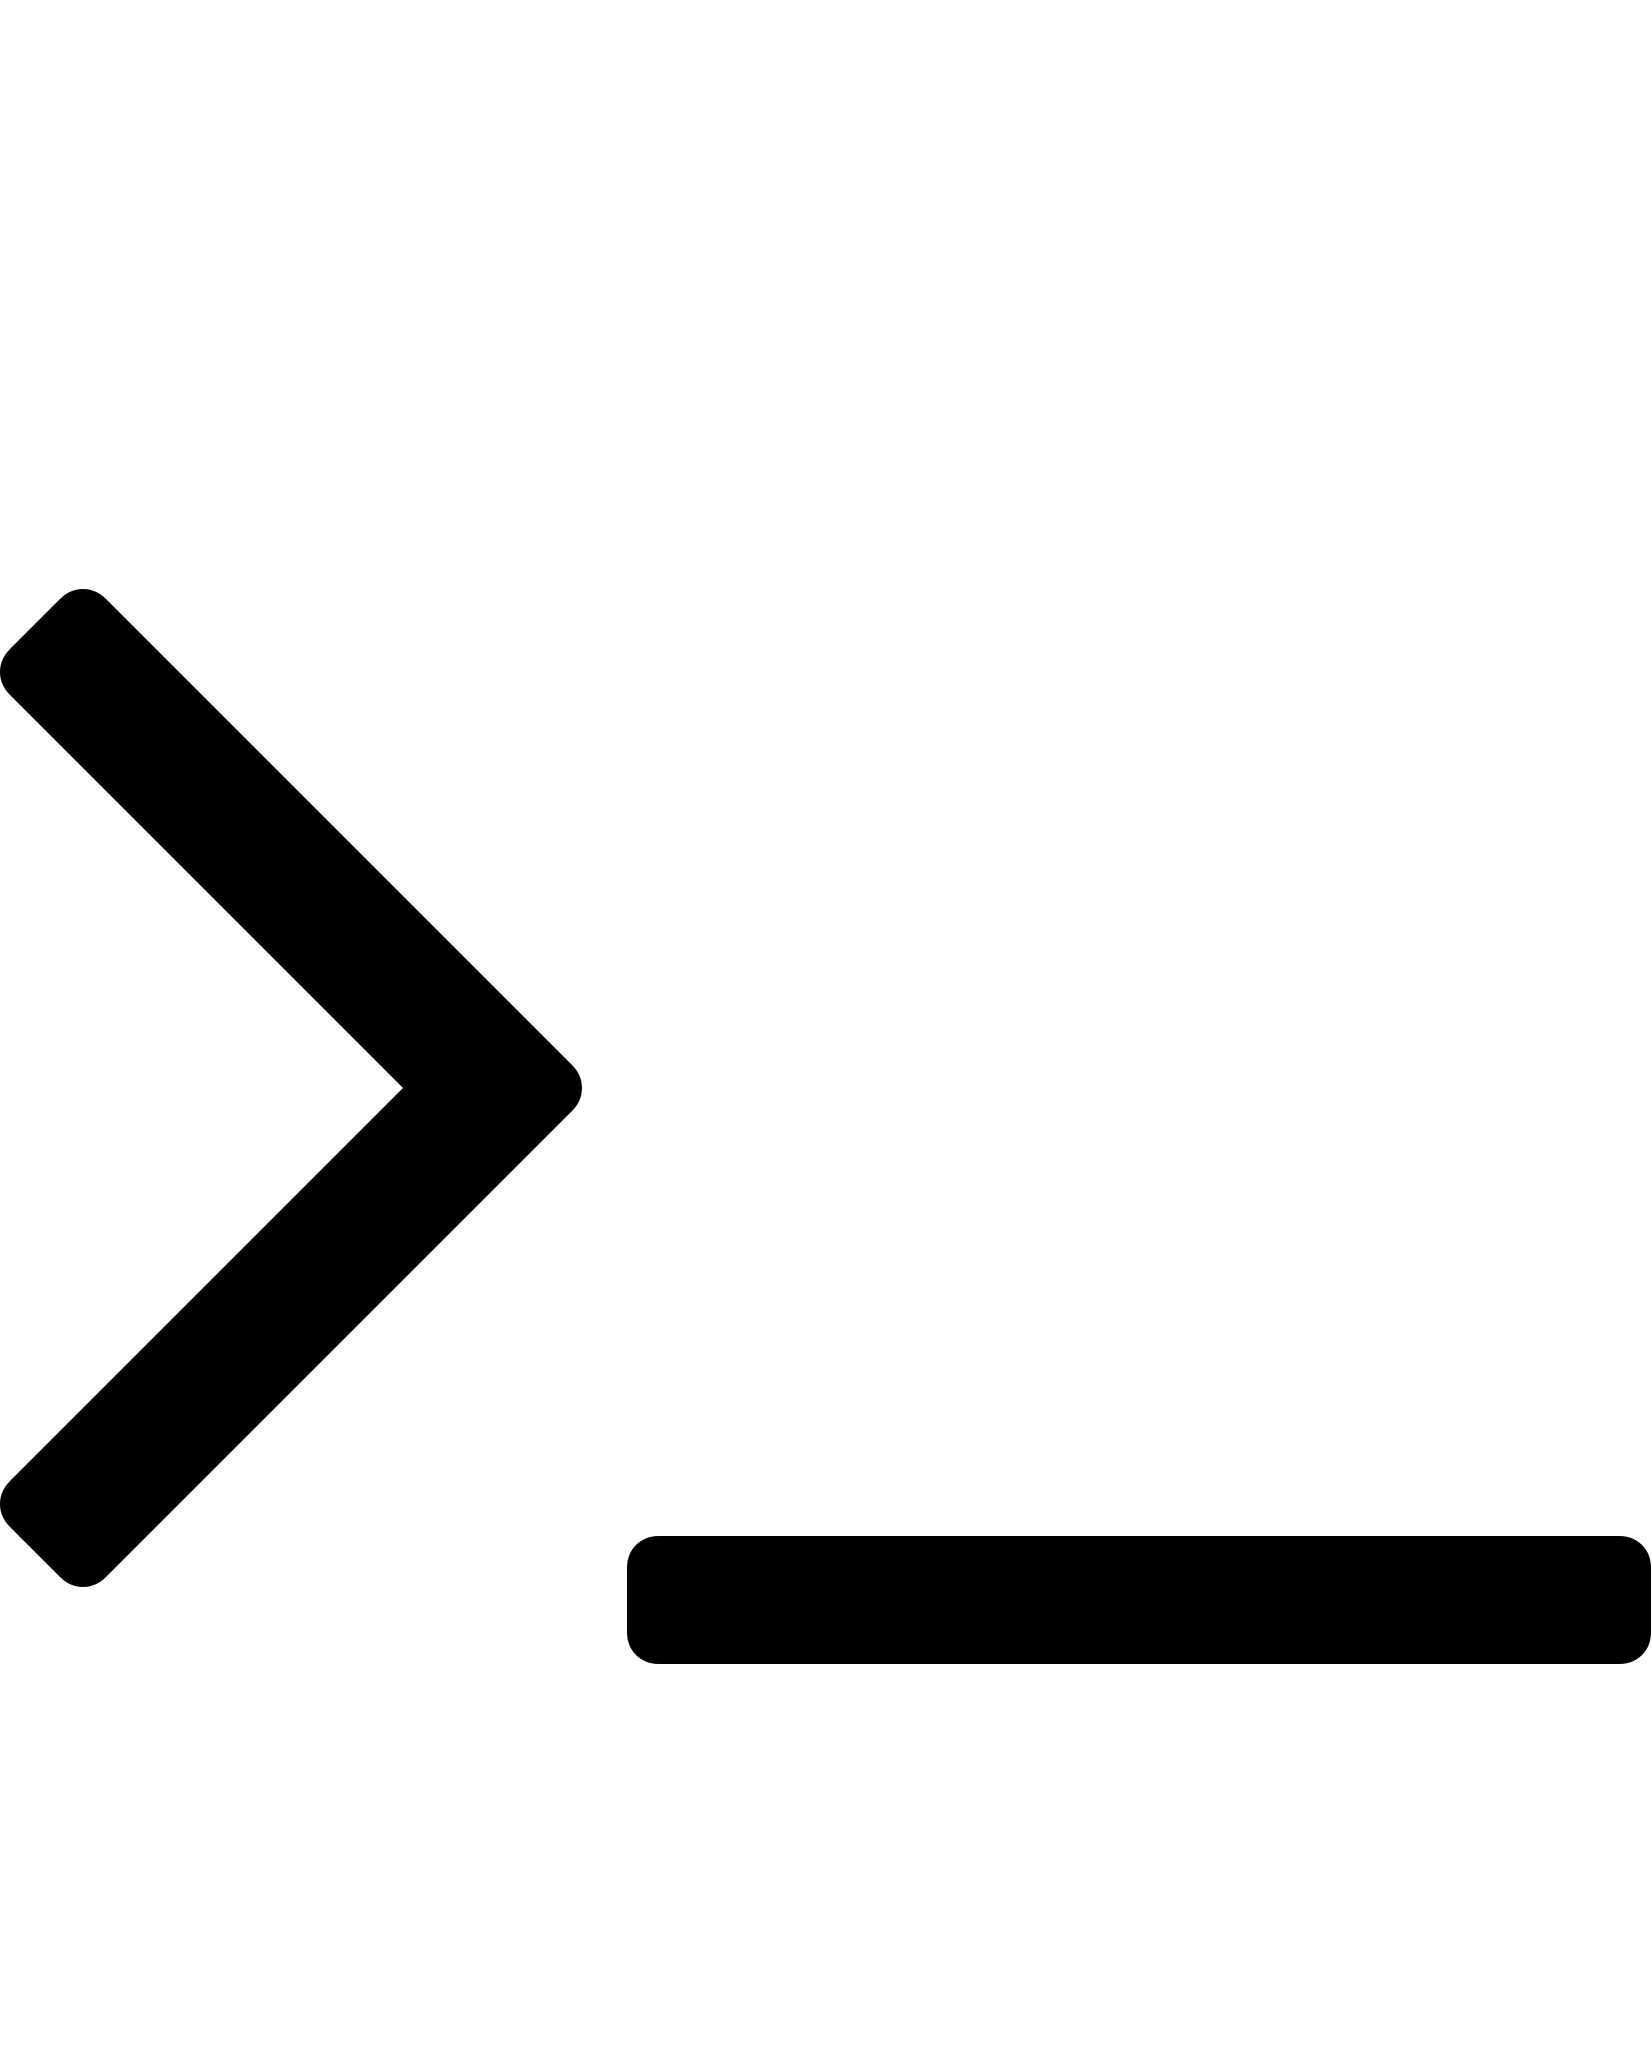
\includegraphics[width=4cm]{images/demo}
    \end{center}
  \end{frame}

  \section{Bench system}
  \begin{frame}
    \frametitle{Bench system}
    \begin{center}
      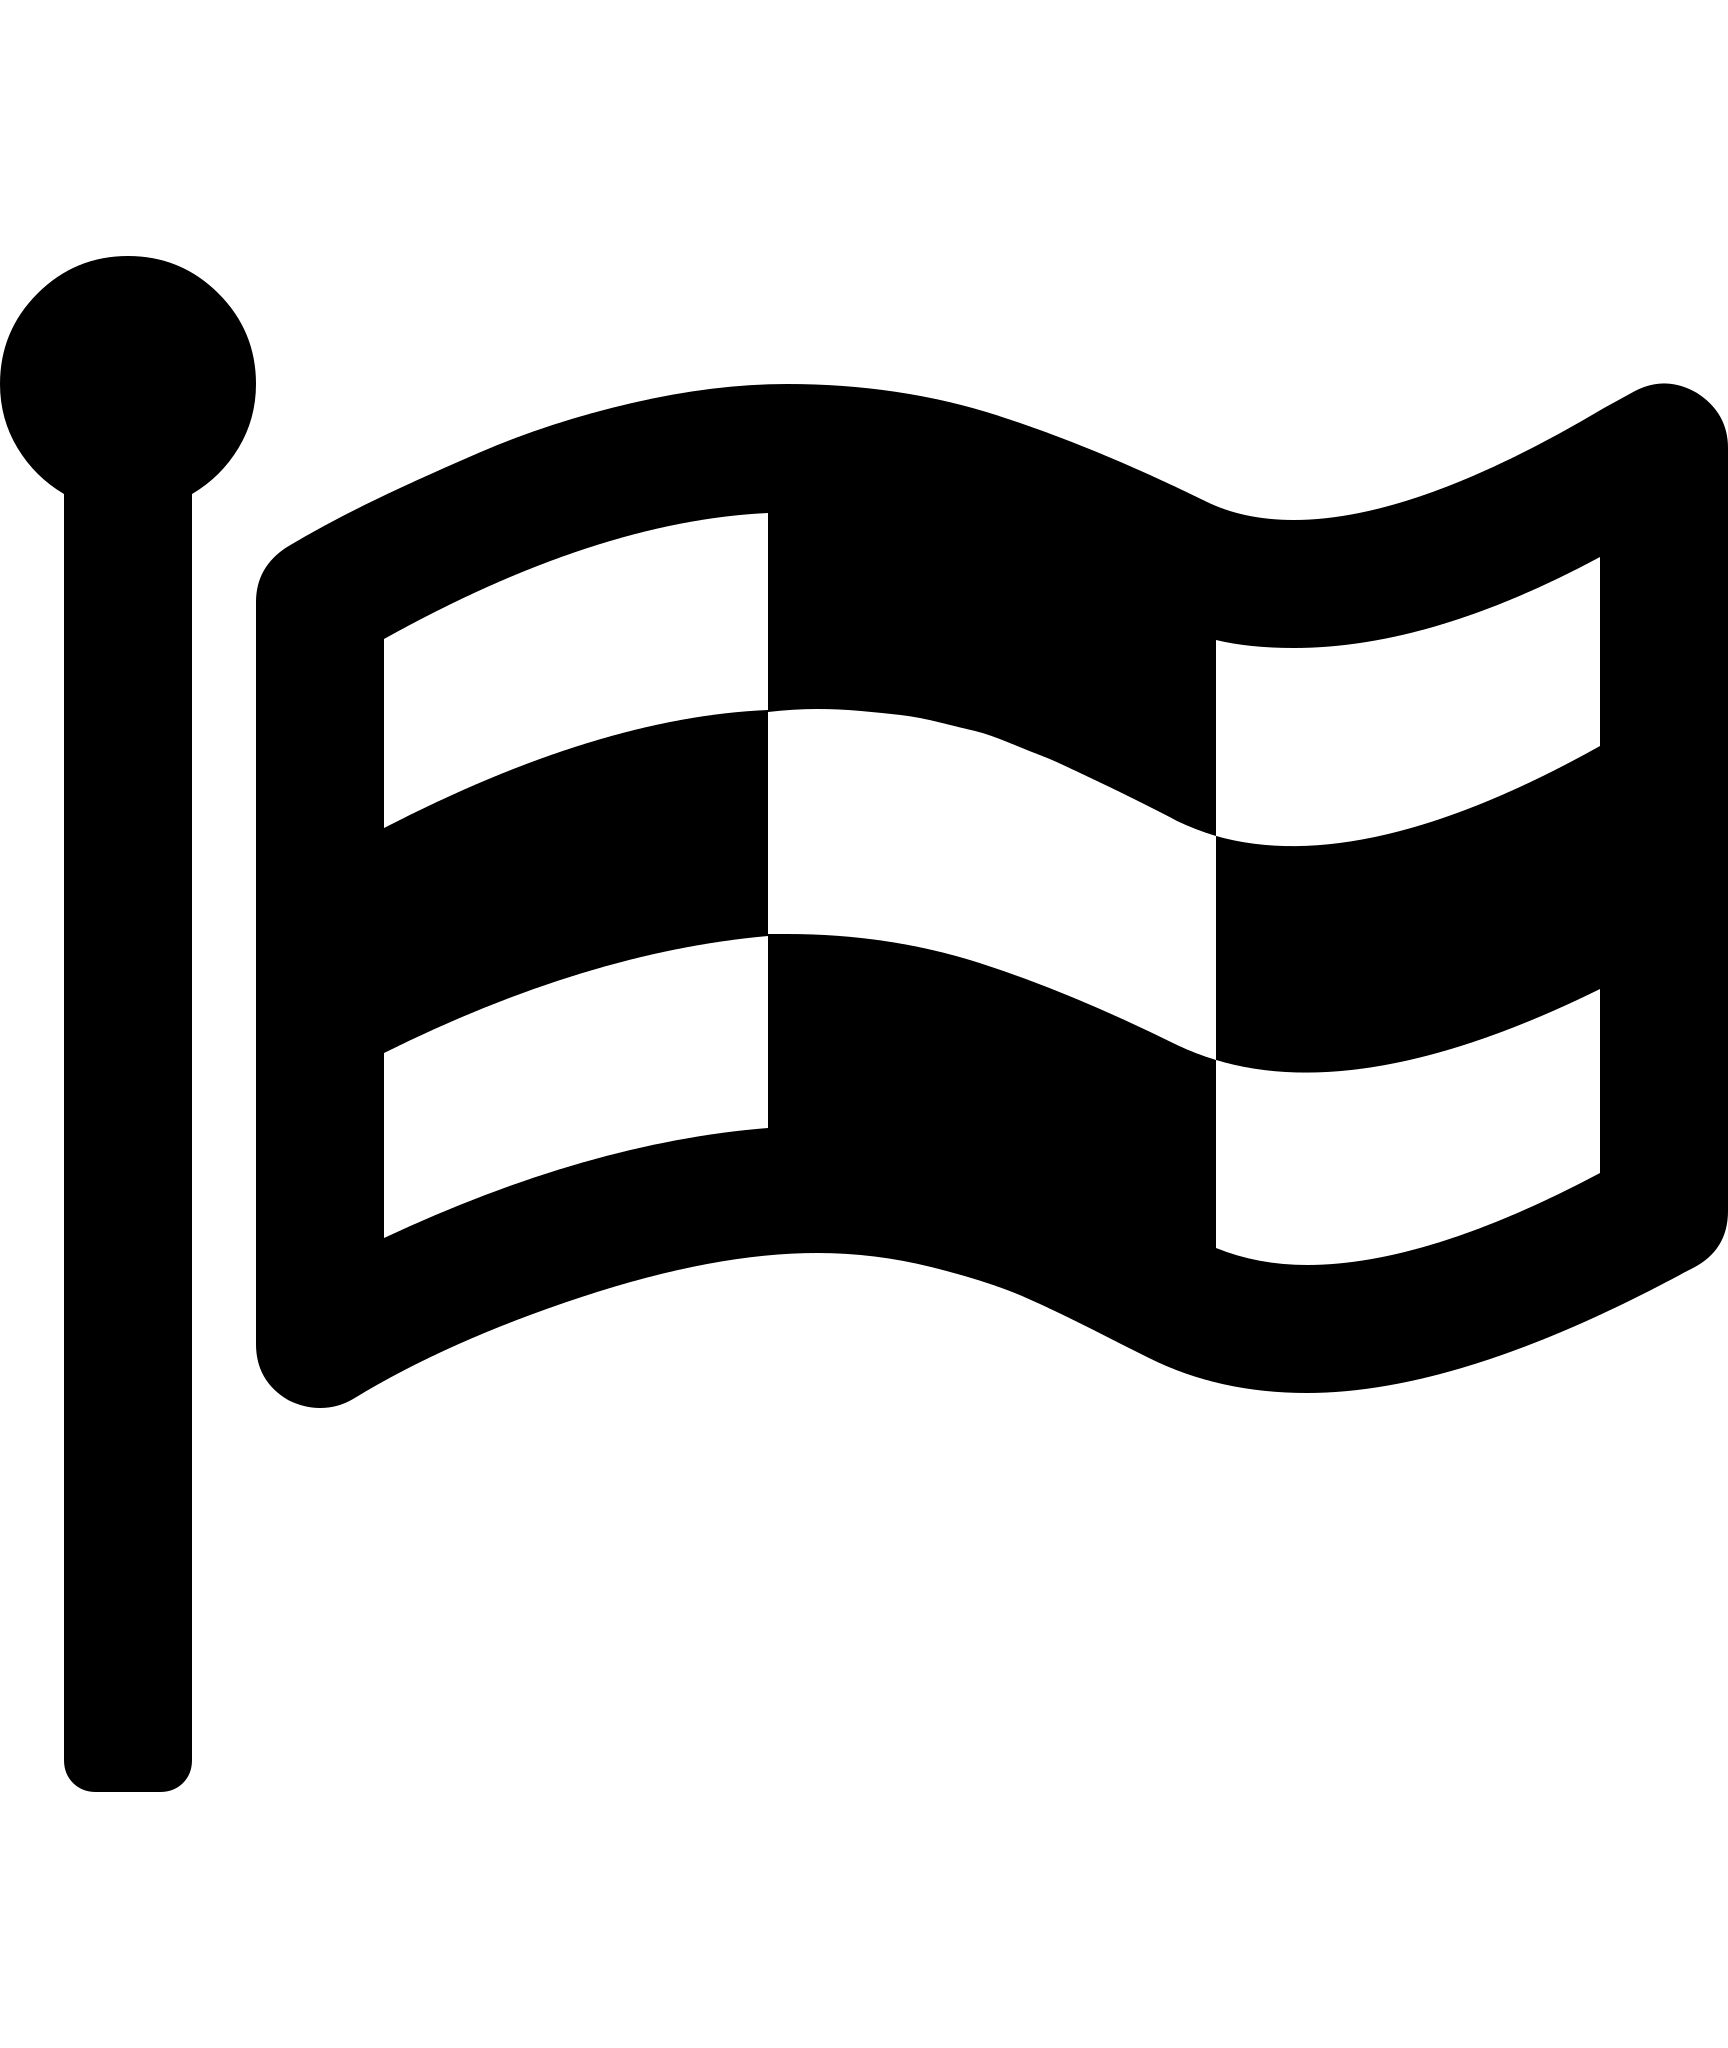
\includegraphics[width=4cm]{images/bench}
    \end{center}
  \end{frame}
\end{document}
